%%%%%%%%%%%%%%%%%%%%%%%%%%%%%%%%%%%%%%%%%
% Journal Article
% LaTeX Template
% Version 1.4 (15/5/16)
%
% This template has been downloaded from:
% http://www.LaTeXTemplates.com
%
% Original author:
% Frits Wenneker (http://www.howtotex.com) with extensive modifications by
% Vel (vel@LaTeXTemplates.com)
%
% License:
% CC BY-NC-SA 3.0 (http://creativecommons.org/licenses/by-nc-sa/3.0/)
%
%%%%%%%%%%%%%%%%%%%%%%%%%%%%%%%%%%%%%%%%%

%----------------------------------------------------------------------------------------
%	PACKAGES AND OTHER DOCUMENT CONFIGURATIONS
%----------------------------------------------------------------------------------------

\documentclass[twoside, twocolumn]{article}

%\usepackage[sc]{mathpazo} % Use the Palatino font
%\usepackage[UTF8]{fontenc} % Use 8-bit encoding that has 256 glyphs
\linespread{1.05} % Line spacing - Palatino needs more space between lines
\usepackage{microtype} % Slightly tweak font spacing for aesthetics
\usepackage[english]{babel} % Language hyphenation and typographical rules
\usepackage{amsmath}

\usepackage[hmarginratio=1:1,top=1in,left=1in,columnsep=20pt]{geometry} % Document margins
\usepackage[hang, small,labelfont=bf,up,textfont=it,up]{caption} % Custom captions under/above floats in tables or figures
\usepackage{booktabs} % Horizontal rules in tables

\usepackage{lettrine} % The lettrine is the first enlarged letter at the beginning of the text

\usepackage{enumitem} % Customized lists
\setlist[itemize]{noitemsep} % Make itemize lists more compact

\usepackage{abstract} % Allows abstract customization
\renewcommand{\abstractnamefont}{\normalfont\bfseries} % Set the "Abstract" text to bold
\renewcommand{\abstracttextfont}{\normalfont\small\itshape} % Set the abstract itself to small italic text

\usepackage{titlesec} % Allows customization of titles
\renewcommand\thesection{\Roman{section}} % Roman numerals for the sections
\renewcommand\thesubsection{\alph{subsection}} % roman numerals for subsections
\titleformat{\section}[block]{\large\scshape\centering}{\thesection.}{1em}{} % Change the look of the section titles
\titleformat{\subsection}{\itshape\bfseries}{\thesubsection.}{1ex}{} % Change the look of the section titles

% \usepackage{fancyhdr} % Headers and footers
% \pagestyle{fancy} % All pages have headers and footers
% \fancyhead{} % Blank out the default header
% \fancyfoot{} % Blank out the default footer
% %\fancyhead[C]{Running title $\bullet$ May 2016 $\bullet$ Vol. XXI, No. 1} % Custom header text
% \fancyfoot[RO,LE]{\thepage} % Custom footer text

\usepackage{titling} % Customizing the title section
\usepackage{hyperref} % For hyperlinks in the PDF
%\usepackage{flushend}
\usepackage{tabularx}
\usepackage{listings}
\usepackage{xcolor}
\usepackage{graphicx}
\usepackage{gensymb}
\usepackage{multirow}
\usepackage{stackengine}


\renewcommand{\c}{\text{c}}
\newcommand{\s}{\text{s}}
\newcommand{\pihalf}{\frac{\pi}{2}}
\newcommand{\T}[2]{\mbox{$_{#2}^{#1}{T}$}}
\newcommand{\R}[2]{\mbox{$_{#2}^{#1}{R}$}}
\newcommand{\code}[1]{{\texttt{#1}}}
\newcommand{\acos}{\text{acos}}
\newcommand{\asin}{\text{asin}}
\newcommand{\figref}[1]{Fig.~\ref{fig:#1}}
\newcommand{\tabref}[1]{Tab.~\ref{tab:#1}}

\def\stackalignment{l}
\newcommand{\imgframe}[2]{\topinset{\colorbox{black}{\textcolor{white}{#2}}}{\includegraphics[width=0.25\linewidth]{img/#1-#2.png}}{0cm}{0cm}}


\lstset{
  %frame=tb,
  language=Python,
  aboveskip=3mm,
  belowskip=3mm,
  showstringspaces=false,
  columns=flexible,
  basicstyle={\small\ttfamily},
  numbers=none,
  % numberstyle=\tiny\color{gray},
  % keywordstyle=\color{blue},
  % commentstyle=\color{dkgreen},
  % stringstyle=\color{mauve},
  breaklines=true,
  breakatwhitespace=true,
  tabsize=3
}
%----------------------------------------------------------------------------------------
%	TITLE SECTION
%----------------------------------------------------------------------------------------

\setlength{\droptitle}{-4\baselineskip} % Move the title up

\pretitle{\begin{center}\Huge\bfseries} % Article title formatting
\posttitle{\end{center}} % Article title closing formatting
\title{RoboND "Follow Me" Project Report   } % Article title
\author{%
\textsc{Wolfgang Steiner} \\[0.5ex] % Your name
%\normalsize University of California \\ % Your institution
\normalsize \href{mailto:wolfgang.steiner@gmail.com}{wolfgang.steiner@gmail.com} % Your email address
%\and % Uncomment if 2 authors are required, duplicate these 4 lines if more
%\textsc{Jane Smith}\thanks{Corresponding author} \\[1ex] % Second author's name
%\normalsize University of Utah \\ % Second author's institution
%\normalsize \href{mailto:jane@smith.com}{jane@smith.com} % Second author's email address
}
\date{\today} % Leave empty to omit a date
\renewcommand{\maketitlehookd}{%
% \begin{abstract}
% \noindent
% \end{abstract}
}

%----------------------------------------------------------------------------------------

\begin{document}

% Print the title
\maketitle

%-------------------------------------------------------------------------------------------
%	ARTICLE CONTENTS
%-------------------------------------------------------------------------------------------
%%%%%%%%%%%%%%%%%%%%%%%%%%%%%%%%%%%%%%%%%%%%%%%%%%%%%%%%%%%%%%%%%%%%%%%%%%%%%%%%%%%%%%%%%%%%%%%%
\section{Introduction}
In this project I trained a fully-convolutional neural network in order to
perform semantic scene segmentation on images obtained from simulation. The
aim is to distinguish a target object from the scene background and from other
non-target objects in order to follow it with a robotic drone.

\section{Network Architecture}
The network architecture of the fully convolutional network used in this project
is shown in \figref{model}. Following the input layer, three convolutional encoders reduce
the size of the input image by a factor of two each, while the filter size of each
layer increases in order to encode the feature vectors for the image segmentation.
The encoders consist of a convolution followed by a batch normalization layer which
ensures faster learning progress by re-normalizing the feature vectors for each
batch during training. In the network with the highest accuracy the first encoder
has a filter depth of 64 which is doubled for the deeper encoders.

The encoder layers are followed by a 1x1 convolution with a filter depth of
256. \textbf{This convolutional layer is used instead of a fully connected layer in order
to retain the spacial information of the segmented image.}
After this layer, three decoder layers are used to interpolate the segmentation
back to the resolution of the input image. Each decoder uses bilinear interpolation
to increase the resolution by a factor of two. Additionally, a second input is
concatenated with the up-sampled tensor. This measure ensures that the network is
able to do image segmentation at different scale or resolution levels.


\textbf{The output layer consists of a dense layer with softmax activation function. It has
three output classes for background, target object and other object. Thus the fully-connected
output layer will be able to classify each of the pixels in the image as one
of three output classes.}

\begin{figure}[ht]
\centering
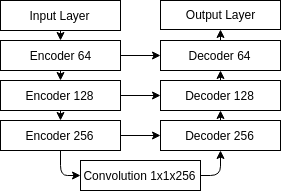
\includegraphics[width=0.75\columnwidth]{fig/model_alt.png}
\caption{\label{fig:model} Model architecture of the fully convolutional neural network.}
\end{figure}

\section{Training Procedure}
\subsection{Optimizer and Learning Rate}
As an optimizer for training I chose the Adam algorithm which. The learning
rate determines the step size during gradient descent. We would want the learning
rate to be high in order to make fast progress during training. But if the
learning rate is chosen too high, training might not converge. Choosing a learining
rate that is too low might result in the training getting stuck in a local
minimum which would not result in the best model possible. This problem is mitigated
when using the Adam optimizer because it will dynamically adjust the training rate
as the training progresses. From experience, I chose 0.001 as the training rate, which
is also the default value for the Adam optimizer in Keras.

\subsection{Training Epoch}
The training epoch is an arbitrary convention used in the training of neural networks.
Commonly one epoch is counted when all of the training examples have been used
once during optimization. The number of epochs is then a measure of how long
the network has been trained on the training data. After each epoch, the
validation loss is calculated by evaluating the validation images. I did not chose
a specific number of epochs for training. I defined a maximum number of epochs
of 64 for training. By using a checkpoint callback, the model was saved every time
the validation loss decreased.

\subsection{Batch Size}
The batch size determines how many training examples are used in for one step of
the optimization procedure. Here a balance must be achieved between convergence
on the one hand which commonly favors smaller batch sizes and parallelization on
the GPU which calls for larger batch sizes. I picked 32 as a batch size and found
training performance to be good. Thus I did not have a reason to change or
experiment with this value.

\subsection{Data Augmentation}
I implemented a simple data augmentation procedure which randomly flips the training and
ground truth images horizontally. This kind of data augmentation is very easy
to implement and practically doubles the number of training examples for free.


\section{Results}
The results for different combinations of filter depth and training epochs are
shown in \tabref{results}. Here the filter depth of the first encoder layers are
specified and the filter depth doubled for each succeeding layer. I started out
with a filter size of 16/32/64 and trained the model for 16 epochs. The resulting
accuracy score was 0.318. I then doubled the filter depth to 32/64/128 and achieved
a score of 0.365.

At this point I introduced data augmentation by horizontal flipping and changed
the training procedure by increasing the maximum number of training epochs while
saving the model after each decrease of the validation loss. With these measures
I was able to achieve a score of 0.445 after 52 epochs. Finally, I increased the filter depth
to 64/128/256 and achieved a score of 0.466 after training the model for 61 epochs.

\begin{table}[ht]
\centering
\caption{\label{tab:results} Model accuracy for different filter depth and number of training epochs.}
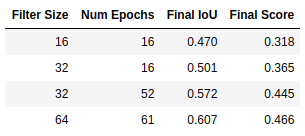
\includegraphics[width=\columnwidth]{fig/results.png}
\end{table}

The learning curves of this final model is shown in \figref{training_curve}. Some
example images containing the target object and other objects are shown in
\figref{segmentation_examples}.

\begin{figure}[ht]
\centering
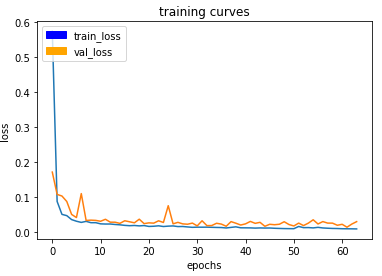
\includegraphics[width=\columnwidth]{fig/training_curve.png}
\caption{\label{fig:training_curve} Training curve of the final model with filter depth 64/128/256.}
\end{figure}

\begin{figure}[ht]
\centering
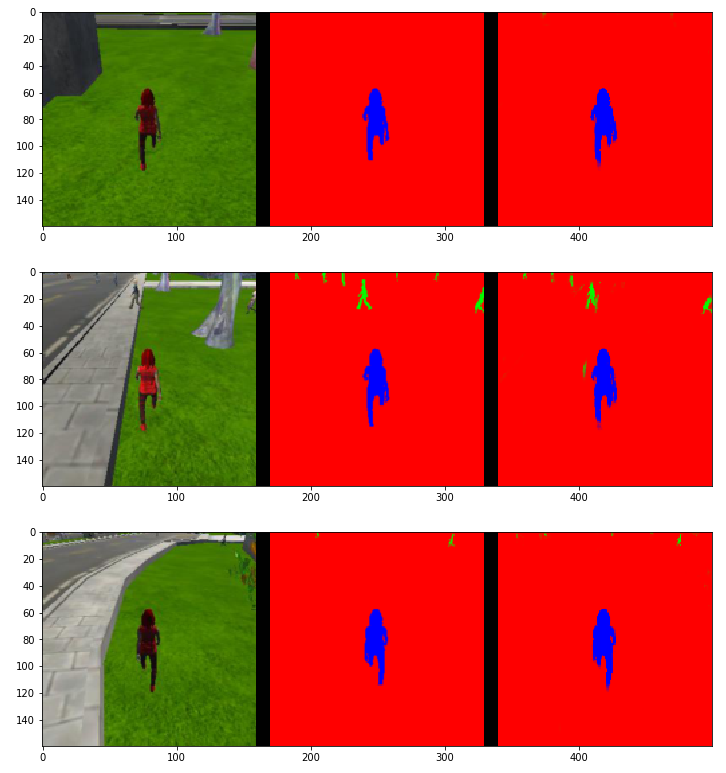
\includegraphics[width=\columnwidth]{fig/segmentation_examples.png}
\caption{\label{fig:segmentation_examples} Sample images from the test set:
Original image (left), ground truth (center), segmentation results (right).}
\end{figure}


\section{Limitations of the Model}
As this model was trained specifically on images derived from a simulator, I would
not expect it to work particularly well on real-world images from a camera. Furthermore,
the target object in the training data was a humanoid dressed in red clothes. Thus,
it would not be possible for the drone to follow other persons dressed in different colors or
even other objects or animals. We could use the same model architecture unchanged but train on
different image data if the task was for the drone to follow one specific object.
I think that it would also be possible to train the same model to classify different
objects as a target but then the model would follow any of the object classified as "target"
indiscriminately. If the drone should be able to select one specific target object from
a collection of targets, the number of classes would need to be altered. This could
be achieved by changing the number of output neurons of the final dense layer of the
model.

\section{Future Enhancements}
In order to improve the accuracy of the model, the filter depth could be further increased
for both the encoder and the decoder layers. Also it would be worthwhile to investigate
whether additional layers would increase segmentation accuracy. Of course, collecting
additional data would be advantageous as would be a more elaborate implementation
of data augmentation. Images could be slightly rotated or skewed and the lighting could be
adjusted on the training images.

%----------------------------------------------------------------------------------------
%	REFERENCE LIST
%----------------------------------------------------------------------------------------
%\bibliography{main}
%\bibliographystyle{ieeetr}
%----------------------------------------------------------------------------------------

\end{document}
